\section{Work plan}
We held many meetings throughout the term on the subject of planning and task division. On average, we would meet once every week or two to modify design decisions and evolve the architecture. Whiteboarding of the design and architecture was documented.

\subsection{Timeline}
Cumulatively, we logged over 450 hours on this prototype. Figure~\ref{fig:work-per-week} shows the week-by-week breakdown. On average, we spent 38.125 hours building the prototype. 

\begin{figure}[tbph]
  \centering
  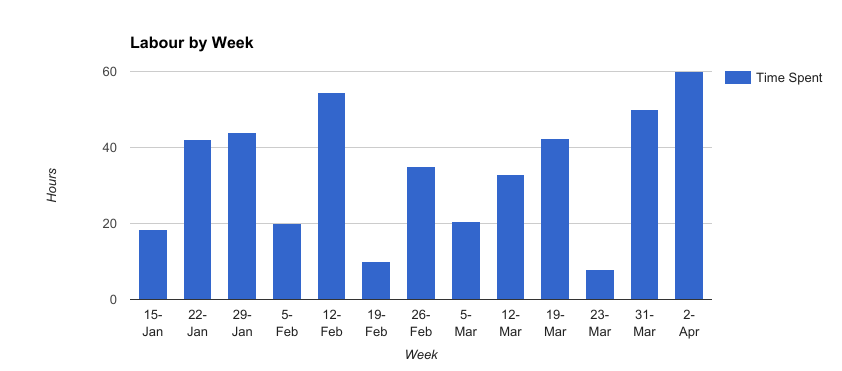
\includegraphics[width=0.85\linewidth]{graphics/work-per-week}
  \caption{Work per week on prototype, all tasks}
  \label{fig:work-per-week}
\end{figure}

Figure~\ref{fig:work-pie} shows that over half of the work time was spent on implementation. Design sessions took the form of collaborative whiteboarding and brainstorming activities with the group as a whole. 

\begin{figure}[tbph]
  \centering
  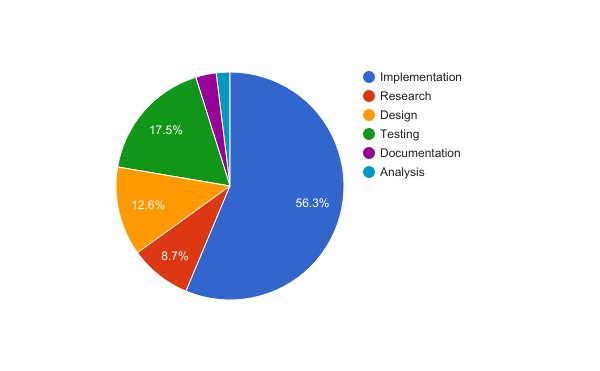
\includegraphics[width=0.7\linewidth]{graphics/work-pie}
  \caption{Areas of work}
  \label{fig:work-pie}
\end{figure}

System testing was almost exclusively through code review, where implementations were examined by other group members for output validity and code quality.


